\documentclass[a4paper,17pt]{extarticle}


    \usepackage[sfdefault, condensed]{roboto} % police d'écriture plus moderne
\usepackage[french]{babel} % francisation
\usepackage[parfill]{parskip} %suppression indentation

\usepackage{fancyhdr}
\usepackage{multicol}

% figure non flotantes
\usepackage{float}
\let\origfigure\figure
\let\endorigfigure\endfigure
\renewenvironment{figure}[1][2] {
    \expandafter\origfigure\expandafter[H]
} {
    \endorigfigure
}

% mois/année
\usepackage{datetime}
\newdateformat{monthyeardate}{%
  \monthname[\THEMONTH] \THEYEAR}

% couleurs perso
\usepackage[table]{xcolor}
\definecolor{deepblue}{rgb}{0.3,0.3,0.8}
\definecolor{darkblue}{rgb}{0,0,0.3}
\definecolor{deepred}{rgb}{0.6,0,0}
\definecolor{iremred}{RGB}{204,35,50}
\definecolor{deepgreen}{rgb}{0,0.6,0}
\definecolor{backcolor}{rgb}{0.98,0.95,0.95}
\definecolor{grisClair}{rgb}{0.95,0.95,0.95}
\definecolor{orangeamu}{RGB}{250,178,11}
\definecolor{noiramu}{RGB}{35,31,32}
\definecolor{bleuamu}{RGB}{20,118,198}
\definecolor{bleuamudark}{RGB}{15,90,150}
\definecolor{cyanamu}{RGB}{77,198,244}


\usepackage{/home/bouscadilla/Documents/Code/nbconvert/template/latex/pdf_solution/xeboiboites}
%
% exemple
\newbreakabletheorem[
    small box style={fill=deepblue!90,draw=deepblue!15, rounded corners,line width=1pt},%
    big box style={fill=deepblue!5,draw=deepblue!15,thick,rounded corners,line width=1pt},%
    headfont={\color{white}\bfseries}
        ]{exemple}{Exemple}{}%{counterCo}
%
% remarque
\newbreakabletheorem[
    small box style={draw=ansi-green-intense!100,line width=2pt,fill=ansi-green-intense!0,rounded corners,decoration=penciline, decorate},%
	big box style={color=ansi-green-intense!90,fill=ansi-green-intense!10,thick,decoration={penciline},decorate},
    broken edges={draw=ansi-green-intense!90,thick,fill=orange!20!black!5, decoration={random steps, segment length=.5cm,amplitude=1.3mm},decorate},%
    other edges={decoration=penciline,decorate,thick},%
    headfont={\color{ansi-green-intense}\large\scshape\bfseries}
    ]{remarque}{Remarque}{}%{counterCa}
%
% formule (sans titre)
\newboxedequation[%
    big box style={fill=cyanamu!10,draw=cyanamu!100,thick,decoration=penciline,decorate}]%
    {form}
%
% Réponse
\newbreakabletheorem[
    small box style={fill=bleuamu!100, draw=bleuamu!60, line width=1pt,rounded corners,decorate},%
    big box style={fill=bleuamu!10,draw=bleuamu!30,thick,rounded corners,decorate},
    headfont={\color{white}\large\scshape\bfseries}
        ]{reponse}{Correction}{}
%

%
% À retenir
%\newbreakabletheorem[
%    small box style={fill=deepred!100, draw=deepred!80, line width=1pt,rounded corners,decorate},%
%    big box style={fill=deepred!10,draw=deepred!50,thick,rounded corners,decorate},
%    headfont={\color{white}\large\scshape\bfseries}
%        ]{retenir}{À retenir}{}
%
\newboxedequation[%
    big box style={fill=deepred!10,draw=deepred!0,thick,decoration=penciline,decorate}]%
    {retenir}



% astuce
\newspanning[
    image=/home/bouscadilla/Documents/Code/nbconvert/template/latex/pdf_solution/fig-idee,headfont=\bfseries,
    spanning style={very thick,decoration=penciline,decorate}
    ]{astuce}{Astuce}{}
%
% activité

\newcounter{counterCa}
\newbreakabletheorem[
    small box style={draw=orangeamu!100,line width=2pt,fill=orangeamu!100,rounded corners,decoration=penciline, decorate},%
	big box style={color=orangeamu!100,fill=orangeamu!5,thick,decoration={penciline},decorate},
    broken edges={draw=orangeamu!100,thick,fill=orangeamu!100, decoration={random steps, segment length=.5cm,amplitude=1.3mm},decorate},%
    other edges={decoration=penciline,decorate,thick},%
    headfont={\color{white}\large\scshape\bfseries}
    ]{activite}{\adjustimage{height=1cm, valign=m}{/home/bouscadilla/Documents/Code/nbconvert/template/latex/pdf_solution/papier_eleve_investigation.png}%
    Activité}{counterCa}
%   
%   environnement élève
%
\newenvironment{eleve}%
%{\begin{activite}\large\\} % écrire plus gros
{\begin{activite}\color{noiramu}\\[-0.5cm]}
{\end{activite}}

\newenvironment{formule}%
%{\begin{activite}\large\\} % écrire plus gros
{\begin{form}\color{bleuamu}}
{\end{form}}


\usepackage[breakable]{tcolorbox}
    \usepackage{parskip} % Stop auto-indenting (to mimic markdown behaviour)
    
    \usepackage{iftex}
    \ifPDFTeX
    	\usepackage[T1]{fontenc}
    	\usepackage{mathpazo}
    \else
    	\usepackage{fontspec}
    \fi

    % Basic figure setup, for now with no caption control since it's done
    % automatically by Pandoc (which extracts ![](path) syntax from Markdown).
    \usepackage{graphicx}
    % Maintain compatibility with old templates. Remove in nbconvert 6.0
    \let\Oldincludegraphics\includegraphics
    % Ensure that by default, figures have no caption (until we provide a
    % proper Figure object with a Caption API and a way to capture that
    % in the conversion process - todo).
    \usepackage{caption}
    \DeclareCaptionFormat{nocaption}{}
    \captionsetup{format=nocaption,aboveskip=0pt,belowskip=0pt}

    \usepackage[Export]{adjustbox} % Used to constrain images to a maximum size
    \adjustboxset{max size={0.9\linewidth}{0.9\paperheight}}
    \usepackage{float}
    \floatplacement{figure}{H} % forces figures to be placed at the correct location
    \usepackage{xcolor} % Allow colors to be defined
    \usepackage{enumerate} % Needed for markdown enumerations to work
    \usepackage{geometry} % Used to adjust the document margins
    \usepackage{amsmath} % Equations
    \usepackage{amssymb} % Equations
    \usepackage{textcomp} % defines textquotesingle
    % Hack from http://tex.stackexchange.com/a/47451/13684:
    \AtBeginDocument{%
        \def\PYZsq{\textquotesingle}% Upright quotes in Pygmentized code
    }
    \usepackage{upquote} % Upright quotes for verbatim code
    \usepackage{eurosym} % defines \euro
    \usepackage[mathletters]{ucs} % Extended unicode (utf-8) support
    \usepackage{fancyvrb} % verbatim replacement that allows latex

    % The hyperref package gives us a pdf with properly built
    % internal navigation ('pdf bookmarks' for the table of contents,
    % internal cross-reference links, web links for URLs, etc.)
    \usepackage{hyperref}
    % The default LaTeX title has an obnoxious amount of whitespace. By default,
    % titling removes some of it. It also provides customization options.
    \usepackage{titling}
    \usepackage{longtable} % longtable support required by pandoc >1.10
    \usepackage{booktabs}  % table support for pandoc > 1.12.2
    \usepackage[inline]{enumitem} % IRkernel/repr support (it uses the enumerate* environment)
    \usepackage[normalem]{ulem} % ulem is needed to support strikethroughs (\sout)
                                % normalem makes italics be italics, not underlines
    \usepackage{mathrsfs}
    

    
    % Colors for the hyperref package
    \definecolor{urlcolor}{rgb}{0,.145,.698}
    \definecolor{linkcolor}{rgb}{.71,0.21,0.01}
    \definecolor{citecolor}{rgb}{.12,.54,.11}

    % ANSI colors
    \definecolor{ansi-black}{HTML}{3E424D}
    \definecolor{ansi-black-intense}{HTML}{282C36}
    \definecolor{ansi-red}{HTML}{E75C58}
    \definecolor{ansi-red-intense}{HTML}{B22B31}
    \definecolor{ansi-green}{HTML}{00A250}
    \definecolor{ansi-green-intense}{HTML}{007427}
    \definecolor{ansi-yellow}{HTML}{DDB62B}
    \definecolor{ansi-yellow-intense}{HTML}{B27D12}
    \definecolor{ansi-blue}{HTML}{208FFB}
    \definecolor{ansi-blue-intense}{HTML}{0065CA}
    \definecolor{ansi-magenta}{HTML}{D160C4}
    \definecolor{ansi-magenta-intense}{HTML}{A03196}
    \definecolor{ansi-cyan}{HTML}{60C6C8}
    \definecolor{ansi-cyan-intense}{HTML}{258F8F}
    \definecolor{ansi-white}{HTML}{C5C1B4}
    \definecolor{ansi-white-intense}{HTML}{A1A6B2}
    \definecolor{ansi-default-inverse-fg}{HTML}{FFFFFF}
    \definecolor{ansi-default-inverse-bg}{HTML}{000000}

    % commands and environments needed by pandoc snippets
    % extracted from the output of `pandoc -s`
    \providecommand{\tightlist}{%
      \setlength{\itemsep}{0pt}\setlength{\parskip}{0pt}}
    \DefineVerbatimEnvironment{Highlighting}{Verbatim}{commandchars=\\\{\}}
    % Add ',fontsize=\small' for more characters per line
    \newenvironment{Shaded}{}{}
    \newcommand{\KeywordTok}[1]{\textcolor[rgb]{0.00,0.44,0.13}{\textbf{{#1}}}}
    \newcommand{\DataTypeTok}[1]{\textcolor[rgb]{0.56,0.13,0.00}{{#1}}}
    \newcommand{\DecValTok}[1]{\textcolor[rgb]{0.25,0.63,0.44}{{#1}}}
    \newcommand{\BaseNTok}[1]{\textcolor[rgb]{0.25,0.63,0.44}{{#1}}}
    \newcommand{\FloatTok}[1]{\textcolor[rgb]{0.25,0.63,0.44}{{#1}}}
    \newcommand{\CharTok}[1]{\textcolor[rgb]{0.25,0.44,0.63}{{#1}}}
    \newcommand{\StringTok}[1]{\textcolor[rgb]{0.25,0.44,0.63}{{#1}}}
    \newcommand{\CommentTok}[1]{\textcolor[rgb]{0.38,0.63,0.69}{\textit{{#1}}}}
    \newcommand{\OtherTok}[1]{\textcolor[rgb]{0.00,0.44,0.13}{{#1}}}
    \newcommand{\AlertTok}[1]{\textcolor[rgb]{1.00,0.00,0.00}{\textbf{{#1}}}}
    \newcommand{\FunctionTok}[1]{\textcolor[rgb]{0.02,0.16,0.49}{{#1}}}
    \newcommand{\RegionMarkerTok}[1]{{#1}}
    \newcommand{\ErrorTok}[1]{\textcolor[rgb]{1.00,0.00,0.00}{\textbf{{#1}}}}
    \newcommand{\NormalTok}[1]{{#1}}
    
    % Additional commands for more recent versions of Pandoc
    \newcommand{\ConstantTok}[1]{\textcolor[rgb]{0.53,0.00,0.00}{{#1}}}
    \newcommand{\SpecialCharTok}[1]{\textcolor[rgb]{0.25,0.44,0.63}{{#1}}}
    \newcommand{\VerbatimStringTok}[1]{\textcolor[rgb]{0.25,0.44,0.63}{{#1}}}
    \newcommand{\SpecialStringTok}[1]{\textcolor[rgb]{0.73,0.40,0.53}{{#1}}}
    \newcommand{\ImportTok}[1]{{#1}}
    \newcommand{\DocumentationTok}[1]{\textcolor[rgb]{0.73,0.13,0.13}{\textit{{#1}}}}
    \newcommand{\AnnotationTok}[1]{\textcolor[rgb]{0.38,0.63,0.69}{\textbf{\textit{{#1}}}}}
    \newcommand{\CommentVarTok}[1]{\textcolor[rgb]{0.38,0.63,0.69}{\textbf{\textit{{#1}}}}}
    \newcommand{\VariableTok}[1]{\textcolor[rgb]{0.10,0.09,0.49}{{#1}}}
    \newcommand{\ControlFlowTok}[1]{\textcolor[rgb]{0.00,0.44,0.13}{\textbf{{#1}}}}
    \newcommand{\OperatorTok}[1]{\textcolor[rgb]{0.40,0.40,0.40}{{#1}}}
    \newcommand{\BuiltInTok}[1]{{#1}}
    \newcommand{\ExtensionTok}[1]{{#1}}
    \newcommand{\PreprocessorTok}[1]{\textcolor[rgb]{0.74,0.48,0.00}{{#1}}}
    \newcommand{\AttributeTok}[1]{\textcolor[rgb]{0.49,0.56,0.16}{{#1}}}
    \newcommand{\InformationTok}[1]{\textcolor[rgb]{0.38,0.63,0.69}{\textbf{\textit{{#1}}}}}
    \newcommand{\WarningTok}[1]{\textcolor[rgb]{0.38,0.63,0.69}{\textbf{\textit{{#1}}}}}
    
    
    % Define a nice break command that doesn't care if a line doesn't already
    % exist.
    \def\br{\hspace*{\fill} \\* }
    % Math Jax compatibility definitions
    \def\gt{>}
    \def\lt{<}
    \let\Oldtex\TeX
    \let\Oldlatex\LaTeX
    \renewcommand{\TeX}{\textrm{\Oldtex}}
    \renewcommand{\LaTeX}{\textrm{\Oldlatex}}
    % Document parameters
    % Document title
    \title{02-SQL-TDetCours}
    
    
    
    
    
% Pygments definitions
\makeatletter
\def\PY@reset{\let\PY@it=\relax \let\PY@bf=\relax%
    \let\PY@ul=\relax \let\PY@tc=\relax%
    \let\PY@bc=\relax \let\PY@ff=\relax}
\def\PY@tok#1{\csname PY@tok@#1\endcsname}
\def\PY@toks#1+{\ifx\relax#1\empty\else%
    \PY@tok{#1}\expandafter\PY@toks\fi}
\def\PY@do#1{\PY@bc{\PY@tc{\PY@ul{%
    \PY@it{\PY@bf{\PY@ff{#1}}}}}}}
\def\PY#1#2{\PY@reset\PY@toks#1+\relax+\PY@do{#2}}

\expandafter\def\csname PY@tok@w\endcsname{\def\PY@tc##1{\textcolor[rgb]{0.73,0.73,0.73}{##1}}}
\expandafter\def\csname PY@tok@c\endcsname{\let\PY@it=\textit\def\PY@tc##1{\textcolor[rgb]{0.25,0.50,0.50}{##1}}}
\expandafter\def\csname PY@tok@cp\endcsname{\def\PY@tc##1{\textcolor[rgb]{0.74,0.48,0.00}{##1}}}
\expandafter\def\csname PY@tok@k\endcsname{\let\PY@bf=\textbf\def\PY@tc##1{\textcolor[rgb]{0.00,0.50,0.00}{##1}}}
\expandafter\def\csname PY@tok@kp\endcsname{\def\PY@tc##1{\textcolor[rgb]{0.00,0.50,0.00}{##1}}}
\expandafter\def\csname PY@tok@kt\endcsname{\def\PY@tc##1{\textcolor[rgb]{0.69,0.00,0.25}{##1}}}
\expandafter\def\csname PY@tok@o\endcsname{\def\PY@tc##1{\textcolor[rgb]{0.40,0.40,0.40}{##1}}}
\expandafter\def\csname PY@tok@ow\endcsname{\let\PY@bf=\textbf\def\PY@tc##1{\textcolor[rgb]{0.67,0.13,1.00}{##1}}}
\expandafter\def\csname PY@tok@nb\endcsname{\def\PY@tc##1{\textcolor[rgb]{0.00,0.50,0.00}{##1}}}
\expandafter\def\csname PY@tok@nf\endcsname{\def\PY@tc##1{\textcolor[rgb]{0.00,0.00,1.00}{##1}}}
\expandafter\def\csname PY@tok@nc\endcsname{\let\PY@bf=\textbf\def\PY@tc##1{\textcolor[rgb]{0.00,0.00,1.00}{##1}}}
\expandafter\def\csname PY@tok@nn\endcsname{\let\PY@bf=\textbf\def\PY@tc##1{\textcolor[rgb]{0.00,0.00,1.00}{##1}}}
\expandafter\def\csname PY@tok@ne\endcsname{\let\PY@bf=\textbf\def\PY@tc##1{\textcolor[rgb]{0.82,0.25,0.23}{##1}}}
\expandafter\def\csname PY@tok@nv\endcsname{\def\PY@tc##1{\textcolor[rgb]{0.10,0.09,0.49}{##1}}}
\expandafter\def\csname PY@tok@no\endcsname{\def\PY@tc##1{\textcolor[rgb]{0.53,0.00,0.00}{##1}}}
\expandafter\def\csname PY@tok@nl\endcsname{\def\PY@tc##1{\textcolor[rgb]{0.63,0.63,0.00}{##1}}}
\expandafter\def\csname PY@tok@ni\endcsname{\let\PY@bf=\textbf\def\PY@tc##1{\textcolor[rgb]{0.60,0.60,0.60}{##1}}}
\expandafter\def\csname PY@tok@na\endcsname{\def\PY@tc##1{\textcolor[rgb]{0.49,0.56,0.16}{##1}}}
\expandafter\def\csname PY@tok@nt\endcsname{\let\PY@bf=\textbf\def\PY@tc##1{\textcolor[rgb]{0.00,0.50,0.00}{##1}}}
\expandafter\def\csname PY@tok@nd\endcsname{\def\PY@tc##1{\textcolor[rgb]{0.67,0.13,1.00}{##1}}}
\expandafter\def\csname PY@tok@s\endcsname{\def\PY@tc##1{\textcolor[rgb]{0.73,0.13,0.13}{##1}}}
\expandafter\def\csname PY@tok@sd\endcsname{\let\PY@it=\textit\def\PY@tc##1{\textcolor[rgb]{0.73,0.13,0.13}{##1}}}
\expandafter\def\csname PY@tok@si\endcsname{\let\PY@bf=\textbf\def\PY@tc##1{\textcolor[rgb]{0.73,0.40,0.53}{##1}}}
\expandafter\def\csname PY@tok@se\endcsname{\let\PY@bf=\textbf\def\PY@tc##1{\textcolor[rgb]{0.73,0.40,0.13}{##1}}}
\expandafter\def\csname PY@tok@sr\endcsname{\def\PY@tc##1{\textcolor[rgb]{0.73,0.40,0.53}{##1}}}
\expandafter\def\csname PY@tok@ss\endcsname{\def\PY@tc##1{\textcolor[rgb]{0.10,0.09,0.49}{##1}}}
\expandafter\def\csname PY@tok@sx\endcsname{\def\PY@tc##1{\textcolor[rgb]{0.00,0.50,0.00}{##1}}}
\expandafter\def\csname PY@tok@m\endcsname{\def\PY@tc##1{\textcolor[rgb]{0.40,0.40,0.40}{##1}}}
\expandafter\def\csname PY@tok@gh\endcsname{\let\PY@bf=\textbf\def\PY@tc##1{\textcolor[rgb]{0.00,0.00,0.50}{##1}}}
\expandafter\def\csname PY@tok@gu\endcsname{\let\PY@bf=\textbf\def\PY@tc##1{\textcolor[rgb]{0.50,0.00,0.50}{##1}}}
\expandafter\def\csname PY@tok@gd\endcsname{\def\PY@tc##1{\textcolor[rgb]{0.63,0.00,0.00}{##1}}}
\expandafter\def\csname PY@tok@gi\endcsname{\def\PY@tc##1{\textcolor[rgb]{0.00,0.63,0.00}{##1}}}
\expandafter\def\csname PY@tok@gr\endcsname{\def\PY@tc##1{\textcolor[rgb]{1.00,0.00,0.00}{##1}}}
\expandafter\def\csname PY@tok@ge\endcsname{\let\PY@it=\textit}
\expandafter\def\csname PY@tok@gs\endcsname{\let\PY@bf=\textbf}
\expandafter\def\csname PY@tok@gp\endcsname{\let\PY@bf=\textbf\def\PY@tc##1{\textcolor[rgb]{0.00,0.00,0.50}{##1}}}
\expandafter\def\csname PY@tok@go\endcsname{\def\PY@tc##1{\textcolor[rgb]{0.53,0.53,0.53}{##1}}}
\expandafter\def\csname PY@tok@gt\endcsname{\def\PY@tc##1{\textcolor[rgb]{0.00,0.27,0.87}{##1}}}
\expandafter\def\csname PY@tok@err\endcsname{\def\PY@bc##1{\setlength{\fboxsep}{0pt}\fcolorbox[rgb]{1.00,0.00,0.00}{1,1,1}{\strut ##1}}}
\expandafter\def\csname PY@tok@kc\endcsname{\let\PY@bf=\textbf\def\PY@tc##1{\textcolor[rgb]{0.00,0.50,0.00}{##1}}}
\expandafter\def\csname PY@tok@kd\endcsname{\let\PY@bf=\textbf\def\PY@tc##1{\textcolor[rgb]{0.00,0.50,0.00}{##1}}}
\expandafter\def\csname PY@tok@kn\endcsname{\let\PY@bf=\textbf\def\PY@tc##1{\textcolor[rgb]{0.00,0.50,0.00}{##1}}}
\expandafter\def\csname PY@tok@kr\endcsname{\let\PY@bf=\textbf\def\PY@tc##1{\textcolor[rgb]{0.00,0.50,0.00}{##1}}}
\expandafter\def\csname PY@tok@bp\endcsname{\def\PY@tc##1{\textcolor[rgb]{0.00,0.50,0.00}{##1}}}
\expandafter\def\csname PY@tok@fm\endcsname{\def\PY@tc##1{\textcolor[rgb]{0.00,0.00,1.00}{##1}}}
\expandafter\def\csname PY@tok@vc\endcsname{\def\PY@tc##1{\textcolor[rgb]{0.10,0.09,0.49}{##1}}}
\expandafter\def\csname PY@tok@vg\endcsname{\def\PY@tc##1{\textcolor[rgb]{0.10,0.09,0.49}{##1}}}
\expandafter\def\csname PY@tok@vi\endcsname{\def\PY@tc##1{\textcolor[rgb]{0.10,0.09,0.49}{##1}}}
\expandafter\def\csname PY@tok@vm\endcsname{\def\PY@tc##1{\textcolor[rgb]{0.10,0.09,0.49}{##1}}}
\expandafter\def\csname PY@tok@sa\endcsname{\def\PY@tc##1{\textcolor[rgb]{0.73,0.13,0.13}{##1}}}
\expandafter\def\csname PY@tok@sb\endcsname{\def\PY@tc##1{\textcolor[rgb]{0.73,0.13,0.13}{##1}}}
\expandafter\def\csname PY@tok@sc\endcsname{\def\PY@tc##1{\textcolor[rgb]{0.73,0.13,0.13}{##1}}}
\expandafter\def\csname PY@tok@dl\endcsname{\def\PY@tc##1{\textcolor[rgb]{0.73,0.13,0.13}{##1}}}
\expandafter\def\csname PY@tok@s2\endcsname{\def\PY@tc##1{\textcolor[rgb]{0.73,0.13,0.13}{##1}}}
\expandafter\def\csname PY@tok@sh\endcsname{\def\PY@tc##1{\textcolor[rgb]{0.73,0.13,0.13}{##1}}}
\expandafter\def\csname PY@tok@s1\endcsname{\def\PY@tc##1{\textcolor[rgb]{0.73,0.13,0.13}{##1}}}
\expandafter\def\csname PY@tok@mb\endcsname{\def\PY@tc##1{\textcolor[rgb]{0.40,0.40,0.40}{##1}}}
\expandafter\def\csname PY@tok@mf\endcsname{\def\PY@tc##1{\textcolor[rgb]{0.40,0.40,0.40}{##1}}}
\expandafter\def\csname PY@tok@mh\endcsname{\def\PY@tc##1{\textcolor[rgb]{0.40,0.40,0.40}{##1}}}
\expandafter\def\csname PY@tok@mi\endcsname{\def\PY@tc##1{\textcolor[rgb]{0.40,0.40,0.40}{##1}}}
\expandafter\def\csname PY@tok@il\endcsname{\def\PY@tc##1{\textcolor[rgb]{0.40,0.40,0.40}{##1}}}
\expandafter\def\csname PY@tok@mo\endcsname{\def\PY@tc##1{\textcolor[rgb]{0.40,0.40,0.40}{##1}}}
\expandafter\def\csname PY@tok@ch\endcsname{\let\PY@it=\textit\def\PY@tc##1{\textcolor[rgb]{0.25,0.50,0.50}{##1}}}
\expandafter\def\csname PY@tok@cm\endcsname{\let\PY@it=\textit\def\PY@tc##1{\textcolor[rgb]{0.25,0.50,0.50}{##1}}}
\expandafter\def\csname PY@tok@cpf\endcsname{\let\PY@it=\textit\def\PY@tc##1{\textcolor[rgb]{0.25,0.50,0.50}{##1}}}
\expandafter\def\csname PY@tok@c1\endcsname{\let\PY@it=\textit\def\PY@tc##1{\textcolor[rgb]{0.25,0.50,0.50}{##1}}}
\expandafter\def\csname PY@tok@cs\endcsname{\let\PY@it=\textit\def\PY@tc##1{\textcolor[rgb]{0.25,0.50,0.50}{##1}}}

\def\PYZbs{\char`\\}
\def\PYZus{\char`\_}
\def\PYZob{\char`\{}
\def\PYZcb{\char`\}}
\def\PYZca{\char`\^}
\def\PYZam{\char`\&}
\def\PYZlt{\char`\<}
\def\PYZgt{\char`\>}
\def\PYZsh{\char`\#}
\def\PYZpc{\char`\%}
\def\PYZdl{\char`\$}
\def\PYZhy{\char`\-}
\def\PYZsq{\char`\'}
\def\PYZdq{\char`\"}
\def\PYZti{\char`\~}
% for compatibility with earlier versions
\def\PYZat{@}
\def\PYZlb{[}
\def\PYZrb{]}
\makeatother


    % For linebreaks inside Verbatim environment from package fancyvrb. 
    \makeatletter
        \newbox\Wrappedcontinuationbox 
        \newbox\Wrappedvisiblespacebox 
        \newcommand*\Wrappedvisiblespace {\textcolor{red}{\textvisiblespace}} 
        \newcommand*\Wrappedcontinuationsymbol {\textcolor{red}{\llap{\tiny$\m@th\hookrightarrow$}}} 
        \newcommand*\Wrappedcontinuationindent {3ex } 
        \newcommand*\Wrappedafterbreak {\kern\Wrappedcontinuationindent\copy\Wrappedcontinuationbox} 
        % Take advantage of the already applied Pygments mark-up to insert 
        % potential linebreaks for TeX processing. 
        %        {, <, #, %, $, ' and ": go to next line. 
        %        _, }, ^, &, >, - and ~: stay at end of broken line. 
        % Use of \textquotesingle for straight quote. 
        \newcommand*\Wrappedbreaksatspecials {% 
            \def\PYGZus{\discretionary{\char`\_}{\Wrappedafterbreak}{\char`\_}}% 
            \def\PYGZob{\discretionary{}{\Wrappedafterbreak\char`\{}{\char`\{}}% 
            \def\PYGZcb{\discretionary{\char`\}}{\Wrappedafterbreak}{\char`\}}}% 
            \def\PYGZca{\discretionary{\char`\^}{\Wrappedafterbreak}{\char`\^}}% 
            \def\PYGZam{\discretionary{\char`\&}{\Wrappedafterbreak}{\char`\&}}% 
            \def\PYGZlt{\discretionary{}{\Wrappedafterbreak\char`\<}{\char`\<}}% 
            \def\PYGZgt{\discretionary{\char`\>}{\Wrappedafterbreak}{\char`\>}}% 
            \def\PYGZsh{\discretionary{}{\Wrappedafterbreak\char`\#}{\char`\#}}% 
            \def\PYGZpc{\discretionary{}{\Wrappedafterbreak\char`\%}{\char`\%}}% 
            \def\PYGZdl{\discretionary{}{\Wrappedafterbreak\char`\$}{\char`\$}}% 
            \def\PYGZhy{\discretionary{\char`\-}{\Wrappedafterbreak}{\char`\-}}% 
            \def\PYGZsq{\discretionary{}{\Wrappedafterbreak\textquotesingle}{\textquotesingle}}% 
            \def\PYGZdq{\discretionary{}{\Wrappedafterbreak\char`\"}{\char`\"}}% 
            \def\PYGZti{\discretionary{\char`\~}{\Wrappedafterbreak}{\char`\~}}% 
        } 
        % Some characters . , ; ? ! / are not pygmentized. 
        % This macro makes them "active" and they will insert potential linebreaks 
        \newcommand*\Wrappedbreaksatpunct {% 
            \lccode`\~`\.\lowercase{\def~}{\discretionary{\hbox{\char`\.}}{\Wrappedafterbreak}{\hbox{\char`\.}}}% 
            \lccode`\~`\,\lowercase{\def~}{\discretionary{\hbox{\char`\,}}{\Wrappedafterbreak}{\hbox{\char`\,}}}% 
            \lccode`\~`\;\lowercase{\def~}{\discretionary{\hbox{\char`\;}}{\Wrappedafterbreak}{\hbox{\char`\;}}}% 
            \lccode`\~`\:\lowercase{\def~}{\discretionary{\hbox{\char`\:}}{\Wrappedafterbreak}{\hbox{\char`\:}}}% 
            \lccode`\~`\?\lowercase{\def~}{\discretionary{\hbox{\char`\?}}{\Wrappedafterbreak}{\hbox{\char`\?}}}% 
            \lccode`\~`\!\lowercase{\def~}{\discretionary{\hbox{\char`\!}}{\Wrappedafterbreak}{\hbox{\char`\!}}}% 
            \lccode`\~`\/\lowercase{\def~}{\discretionary{\hbox{\char`\/}}{\Wrappedafterbreak}{\hbox{\char`\/}}}% 
            \catcode`\.\active
            \catcode`\,\active 
            \catcode`\;\active
            \catcode`\:\active
            \catcode`\?\active
            \catcode`\!\active
            \catcode`\/\active 
            \lccode`\~`\~ 	
        }
    \makeatother

    \let\OriginalVerbatim=\Verbatim
    \makeatletter
    \renewcommand{\Verbatim}[1][1]{%
        %\parskip\z@skip
        \sbox\Wrappedcontinuationbox {\Wrappedcontinuationsymbol}%
        \sbox\Wrappedvisiblespacebox {\FV@SetupFont\Wrappedvisiblespace}%
        \def\FancyVerbFormatLine ##1{\hsize\linewidth
            \vtop{\raggedright\hyphenpenalty\z@\exhyphenpenalty\z@
                \doublehyphendemerits\z@\finalhyphendemerits\z@
                \strut ##1\strut}%
        }%
        % If the linebreak is at a space, the latter will be displayed as visible
        % space at end of first line, and a continuation symbol starts next line.
        % Stretch/shrink are however usually zero for typewriter font.
        \def\FV@Space {%
            \nobreak\hskip\z@ plus\fontdimen3\font minus\fontdimen4\font
            \discretionary{\copy\Wrappedvisiblespacebox}{\Wrappedafterbreak}
            {\kern\fontdimen2\font}%
        }%
        
        % Allow breaks at special characters using \PYG... macros.
        \Wrappedbreaksatspecials
        % Breaks at punctuation characters . , ; ? ! and / need catcode=\active 	
        \OriginalVerbatim[#1,codes*=\Wrappedbreaksatpunct]%
    }
    \makeatother

    % Exact colors from NB
    \definecolor{incolor}{HTML}{303F9F}
    \definecolor{outcolor}{HTML}{D84315}
    \definecolor{cellborder}{HTML}{CFCFCF}
    \definecolor{cellbackground}{HTML}{F7F7F7}
    
    % prompt
    \makeatletter
    \newcommand{\boxspacing}{\kern\kvtcb@left@rule\kern\kvtcb@boxsep}
    \makeatother
    \newcommand{\prompt}[4]{
        \ttfamily\llap{{\color{#2}[#3]:\hspace{3pt}#4}}\vspace{-\baselineskip}
    }
    

    
\setlength\headheight{30pt}
\setcounter{secnumdepth}{0} % Turns off numbering for sections

    % Prevent overflowing lines due to hard-to-break entities
    \sloppy 
    % Setup hyperref package
    \hypersetup{
      breaklinks=true,  % so long urls are correctly broken across lines
      colorlinks=true,
      urlcolor=urlcolor,
      linkcolor=linkcolor,
      citecolor=citecolor,
      }
    % Slightly bigger margins than the latex defaults
    \geometry{a4paper,tmargin=3cm,bmargin=2cm,lmargin=1cm,rmargin=1cm}\fancyhead[L]{Thème à définir}\fancyhead[L]{\adjustimage{height=1cm, valign=m}{/home/bouscadilla/Documents/Code/nbconvert/template/latex/pdf_solution/papier_eleve_ico_data}\ttfamily\scshape Données}\fancyhead[C]{\bfseries\MakeUppercase{02-SQL-TDetCours}}\fancyhead[C]{\bfseries\MakeUppercase{8 --- Base de donnée relationnelle}}\fancyhead[R]{\monthyeardate\today}

    \fancyfoot[C]{\thepage}
    % #TODO ajouter les pages totales

    \pagestyle{fancy}
    


\begin{document}
    
    \title{8 --- Base de donnée relationnelle}
% \maketitle

    
    

    
    \hypertarget{bases-de-donnuxe9es-relationnelles-en-sql}{%
\section{Bases de données relationnelles en
SQL}\label{bases-de-donnuxe9es-relationnelles-en-sql}}

    \hypertarget{impluxe9mentation-de-contraintes-suppluxe9mentaires}{%
\subsection{Implémentation de contraintes
supplémentaires}\label{impluxe9mentation-de-contraintes-suppluxe9mentaires}}

    Lorsque l'on crée une relation, on peut ajouter des contraintes
d'intégrités autres que clés primaires (\texttt{PRIMARY\ KEY}) ou
étrangères (\texttt{FOREIGN\ KEY\ ...\ REFERENCES\ ...}).

\begin{itemize}
\tightlist
\item
  \texttt{UNIQUE} : la valeur de l'attribut doit être unique
\item
  \texttt{NOT\ NULL} : la valeur de l'attribut de peut pas être laissée
  vide (attention, contrairement à Python la chaîne de caractère vide
  \texttt{\textquotesingle{}\textquotesingle{}} n'est pas égale à
  \texttt{NULL} !)(j'insiste :
  \texttt{\textquotesingle{}\textquotesingle{}} \(\neq\) \texttt{NULL})
\end{itemize}

    Exemple d'utilisation de \texttt{UNIQUE} et \texttt{NOT\ NULL}

\begin{Shaded}
\begin{Highlighting}[]
\KeywordTok{CREATE} \KeywordTok{TABLE}\NormalTok{ livre (titre TEXT }\KeywordTok{NOT} \KeywordTok{NULL}\NormalTok{,}
\NormalTok{                    editeur TEXT }\KeywordTok{NOT} \KeywordTok{NULL}\NormalTok{,}
\NormalTok{                    annee }\DataTypeTok{INTEGER} \KeywordTok{NOT} \KeywordTok{NULL}\NormalTok{,}
\NormalTok{                    isbn TEXT }\KeywordTok{UNIQUE} \KeywordTok{NOT} \KeywordTok{NULL} \KeywordTok{PRIMARY} \KeywordTok{KEY}\NormalTok{);}
\end{Highlighting}
\end{Shaded}

    Remarque : il est redondant d'écrire \texttt{PRIMARY\ KEY} et
\texttt{NOT\ NULL\ UNIQUE}. Cependant, à cause d'un bug de DBeaver avec
SQLITE on prendra la peine d'ajouter explicitement
\texttt{NOT\ NULL\ UNIQUE} pour un attribut de contrainte clé primaire.

    Pour les chaînes de caractères, il existe est possible d'expliciter un
nombre fixe de caractères ou un nombre variable :

\begin{itemize}
\tightlist
\item
  \texttt{VARCHAR(}\(n\)\texttt{)} : chaîne de caractère de taille
  variable d'au plus \(n\) caractères
\item
  \texttt{CHAR(}\(n\)\texttt{)} : chaîne de caractère de taille \(n\)
  (si la valeur est inférieure à n, des espaces sont ajoutées)
\end{itemize}

    Par exemple, on peut explicitement indiquer que l'\texttt{isbn} possède
14 caractères et que \texttt{titre} et \texttt{editeur} du livre ne
dépassent pas 90 caractères de la façon suivante :

\begin{Shaded}
\begin{Highlighting}[]
\KeywordTok{CREATE} \KeywordTok{TABLE}\NormalTok{ livre (titre }\DataTypeTok{VARCHAR}\NormalTok{(}\DecValTok{90}\NormalTok{) }\KeywordTok{NOT} \KeywordTok{NULL}\NormalTok{,}
\NormalTok{                    editeur }\DataTypeTok{VARCHAR}\NormalTok{(}\DecValTok{90}\NormalTok{) }\KeywordTok{NOT} \KeywordTok{NULL}\NormalTok{,}
\NormalTok{                    annee }\DataTypeTok{INTEGER} \KeywordTok{NOT} \KeywordTok{NULL}\NormalTok{,}
\NormalTok{                    isbn }\DataTypeTok{CHAR}\NormalTok{(}\DecValTok{14}\NormalTok{) }\KeywordTok{UNIQUE} \KeywordTok{NOT} \KeywordTok{NULL} \KeywordTok{PRIMARY} \KeywordTok{KEY}\NormalTok{);}
\end{Highlighting}
\end{Shaded}

    \hypertarget{activituxe9-avec-dbeaver}{%
\subsection{Activité avec DBeaver}\label{activituxe9-avec-dbeaver}}

    Vous allez créer votre première base avec DBeaver CE.

\begin{enumerate}
\def\labelenumi{\arabic{enumi}.}
\tightlist
\item
  Créer un fichier vide nommé \texttt{annuaire.db} (par exemple dans un
  terminal, dans le répertoire de votre choix écrire :
  \texttt{touch\ annuaire.db}).
\item
  Ouvrir DBeaver CE
\item
  Créer une nouvelle connexion :

  \begin{enumerate}
  \def\labelenumii{\arabic{enumii}.}
  \tightlist
  \item
    de type SQLite
  \item
    avec \texttt{Browse...}, sélectionner le fichier créé
    \texttt{annuaire.db}.
  \item
    puis \texttt{Terminer}
  \end{enumerate}
\end{enumerate}

    \includegraphics{./img-dbeaver-connexion.png}

    Maintenant que la base est créer, vous pouvez effectuer des requêtes.
Vous allez les écrire dans un fichier où vous pourrez les exécuter
toutes d'un seul coup (peu recommandé), ou ligne par ligne. Comme un
notebook, chaque ligne est un block que vous pouvez exécuter 0, 1 ou
plusieurs fois.

\begin{enumerate}
\def\labelenumi{\arabic{enumi}.}
\tightlist
\item
  \texttt{Éditeur\ SQL\ \textgreater{}\ Nouveau\ script\ SQL}
\item
  écrire par exemple \texttt{CREATE\ TABLE\ test\ (id\ INT);}
\item
  puis positionner le prompt sur la ligne et exécuter l'instruction SQL
  (clic sur le triangle de lecture ou \texttt{CTRL\ +\ Entrée})
\item
  Sauf erreur, la relation \texttt{test} est créée. Pour en être sûr,
  réaliser à nouveau l'étape précédente et normalement il y aura une
  erreur puisque la relation \emph{existe déjà}.
\end{enumerate}

Pour finir avec cette petite prise en main, vous allez insérer des
données et afficher le contenu de la relation :

\begin{enumerate}
\def\labelenumi{\arabic{enumi}.}
\setcounter{enumi}{7}
\tightlist
\item
  Dans une autre ligne du fichier, écrire
  \texttt{INSERT\ INTO\ test\ VALUES\ (1);} et exécuter plusieurs fois
  cette ligne (pour insérer plusieurs fois l'entité \((1)\) dans la
  relation \(test\)).
\item
  Puis écrire et exécuter \texttt{SELECT\ *\ FROM\ test;}.
\end{enumerate}

Si tout s'affiche comme prévu, nous allons voir une dernière
fonctionnalité: afficher le diagramme de la base puis effacer la
relation\ldots{}

\begin{enumerate}
\def\labelenumi{\arabic{enumi}.}
\setcounter{enumi}{9}
\tightlist
\item
  Dans le panneau de gauche de \texttt{annuaire.db}, il doit être
  possible de déplier la base pour voir s'afficher en dessous
  \texttt{Tables\ ;\ Views\ ;\ Indexes\ ;\ Sequences\ ;\ Table\ Triggers\ ;\ Data\ Types}.
\item
  Double-cliquer sur \texttt{Tables}
\item
  Les propriétés des différentes tables (table = \emph{relation})
  s'affichent dans l'onglet \texttt{Propriétés}
\item
  Actualiser la base avec \texttt{F5} puis
\item
  Cliquer sur l'onglet \texttt{ER\ Diagram} pour voir le diagramme de la
  relation.
\item
  Si tout va bien, vous avez quelque chose qui ressemble à cela.
\end{enumerate}

    \includegraphics{./img-dbeaver.png}

    \begin{enumerate}
\def\labelenumi{\arabic{enumi}.}
\tightlist
\item
  Pour finir, vous allez supprimer la relation \texttt{test} de la base
  en exécutant la requête \texttt{DROP\ TABLE\ test;}.
\end{enumerate}

    \hypertarget{activituxe9---retour-sur-annuaire.db}{%
\subsection{\texorpdfstring{Activité - retour sur
\texttt{annuaire.db}}{Activité - retour sur annuaire.db}}\label{activituxe9---retour-sur-annuaire.db}}

    Créer dans la base de donnée \texttt{annuaire.db} l'unique relation
suivante :

\[annuaire (\underline{tel}: String ,  nom: String , prenom: String)\]

Contraintes d'intégrités :

\begin{itemize}
\tightlist
\item
  \(tel\) : clé primaire, non nulle, unique, chaîne de caractère de
  taille variable (100 caracères max)
\item
  \(nom\) : non nul, chaîne de caractère de taille variable (100 max)
\item
  \(prenom\) : non nul , chaîne de caractère de taille variable (20 max)
\end{itemize}

    \hypertarget{impluxe9mentation-des-contraintes-de-domaines-et-nombres-duxe9cimaux}{%
\subsection{Implémentation des contraintes de domaines et nombres
décimaux}\label{impluxe9mentation-des-contraintes-de-domaines-et-nombres-duxe9cimaux}}

    En SQL, on peut ajouter des \textbf{contraintes de domaines}. Par
exemple on peut imposer un attribut \texttt{age} d'être toujours positif
ou nul.

Pour cela, on utilise l'instruction \texttt{CHECK}. Ce qui donne :

\begin{itemize}
\tightlist
\item
  \texttt{CHECK\ (age\ \textgreater{}=\ 0)}
\end{itemize}

On peut utiliser les opérateurs logiques \texttt{NOT}, \texttt{AND} et
\texttt{OR} ainsi que les parenthèses pour les priorités.

    Pour les nombre flottants, il existe un type qui prend en charge le
nombre de chiffres après la virgule et s'occupe des arrondis le cas
échéant.

\begin{itemize}
\tightlist
\item
  \texttt{DECIMAL(}\(c\)\texttt{,}\(d\)\texttt{)} : permet d'afficher un
  nombre de \(c\) chiffres (en tout) dont \(d\) sont après la virgule
\end{itemize}

    Par exemple pour afficher un nombre compris entre 0 et 999 avec une
précision de 3 décimales, on écrira

\texttt{nombre\ DECIMAL(6,\ 3)}

car il y a 6 chiffres en tout dont 3 pour la partie décimale.

    \hypertarget{activituxe9---base-de-donnuxe9e-note.db}{%
\subsection{\texorpdfstring{Activité - base de donnée
\texttt{note.db}}{Activité - base de donnée note.db}}\label{activituxe9---base-de-donnuxe9e-note.db}}

    \hypertarget{cruxe9ation}{%
\subsubsection{Création}\label{cruxe9ation}}

Créer la base de donnée \texttt{note.db} et les trois relations
suivantes :

\begin{itemize}
\tightlist
\item
  \(eleve(nom: String, prenom: String, \underline{num}: String)\)
\item
  \(matiere(intitule: String, \underline{mat\_id}: Int)\)
\item
  \(note(\underline{num\_eleve}: String, \underline{mat\_id}: Int, note: Float)\)
\end{itemize}

    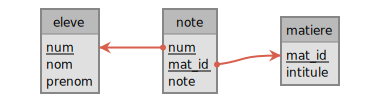
\includegraphics{./img-ex_note.png}

    Attention à respecter les contraintes suivantes :

\begin{itemize}
\tightlist
\item
  \(eleve\) :

  \begin{itemize}
  \tightlist
  \item
    \(nom\) : taille variable (taille 100 max), non nul
  \item
    \(prenom\) : taille variable (max 100), non nul
  \item
    \(num\) : taille variable (max 20), clé primaire (unique, non nul)
  \end{itemize}
\item
  \(matiere\) :

  \begin{itemize}
  \tightlist
  \item
    \(intitule\) : taille variable (max 100), non nul
  \item
    \(mat_id\) : entier, clé primaire (unique non nul)
  \end{itemize}
\item
  \(note\) :

  \begin{itemize}
  \tightlist
  \item
    \(num\_eleve\) : taille variable (max 20), reférence à
    \(eleve(num)\), clé primaire
  \item
    \(mat\_id\) : entier, référence à \(matiere(mat\_id)\), clé primaire
  \item
    \(note\) : nombre décimal de 4 chiffres dont 2 après la virgule, non
    nul, supérieure ou égale à 0, inférieure ou égal à 20
  \end{itemize}
\end{itemize}

    Résultat attendu :

    \includegraphics{./img-ex_note_db.png}

    \hypertarget{suppression}{%
\subsubsection{Suppression}\label{suppression}}

    \begin{enumerate}
\def\labelenumi{\arabic{enumi}.}
\tightlist
\item
  Dans quel ordre faut-il effacer les tables ? Pourquoi ?
\item
  Tester dans DBeaver.
\end{enumerate}

    \hypertarget{activituxe9---base-de-donnuxe9e-vente.db}{%
\subsection{\texorpdfstring{Activité - base de donnée
\texttt{vente.db}}{Activité - base de donnée vente.db}}\label{activituxe9---base-de-donnuxe9e-vente.db}}

    Créer la base de donnée \texttt{vente.db} respectant les contraintes
suivantes :

    \includegraphics{./img-ex_vente.png}

    \hypertarget{ruxe9sumuxe9s-et-notes}{%
\subsection{Résumés et notes}\label{ruxe9sumuxe9s-et-notes}}

    \hypertarget{contraintes}{%
\subsubsection{Contraintes}\label{contraintes}}

\begin{itemize}
\tightlist
\item
  \texttt{PRIMARY\ KEY(auteur\_id)} ou
  \texttt{auteur\_id\ INT\ PRIMARY\ KEY}
\item
  \texttt{PRIMARY\ KEY(auteur\_id,\ isbn)}
\item
  \texttt{FOREIGN\ KEY(auteur\_id)\ REFERENCES\ auteur(a\_id)} ou
  \texttt{auteur\_id\ INT\ REFERENCES\ auteur(a\_id)}
\item
  \texttt{CHECK\ (0\ \textless{}=\ note\ AND\ note\ \textless{}=\ 20)}
\item
  \texttt{CHECK\ (ville\ \textless{}\textgreater{}\ \textquotesingle{}Paris\textquotesingle{})}
  : pour \(\neq\)
\end{itemize}

    \hypertarget{types}{%
\subsubsection{Types}\label{types}}

\begin{itemize}
\tightlist
\item
  \texttt{TEXT} : texte de longueur variable
\item
  \texttt{VARCHAR(}\(n\)\texttt{)} : texte de longueur variable
  inférieure à \(n\)
\item
  \texttt{CHAR(}\(n\)\texttt{)} : texte de longueur \(n\)
\item
  \texttt{INT} ou \texttt{INTEGER} : nombres entiers
\item
  \texttt{DECIMAL(}\(c\)\texttt{,}\(d\)\texttt{)} : nombre flottant de
  \(c\) chiffres dont \(d\) pour la partie décimale
\item
  \texttt{DATE} : une date au format \texttt{AAAA-MM-JJ}
\item
  \texttt{TIME} : une heure au format \texttt{hh:mm:ss}
\item
  \texttt{TIMESTAMP} : un instant (date et heure) au format
  \texttt{AAAA-MM-JJ\ hh:mm:ss}
\end{itemize}

    \hypertarget{tables}{%
\subsubsection{Tables}\label{tables}}

\begin{itemize}
\tightlist
\item
  \texttt{CREATE\ TABLE\ nom\_table\ (...)}
\item
  \texttt{DROP\ TABLE\ nom\_table}
\item
  \texttt{DROP\ TABLE\ IF\ EXISTS\ nom\_table}
\item
  \texttt{INSERT\ INTO\ nom\_table\ VALUES\ (...),\ (...),\ ...,\ ();}
\item
  \texttt{INSERT\ INTO\ nom\_table(attr1,\ attr2)\ VALUES\ ...}
\item
\end{itemize}


    % Add a bibliography block to the postdoc
    
    
    
\end{document}
